\documentclass[10pt]{beamer}
\usepackage{amsmath}
\usepackage{mathtools}
\usepackage{multimedia}
\usepackage{hyperref}


\usefonttheme{professionalfonts} % using non standard fonts for beamer
\usefonttheme{serif} % default family is serif
%\documentclass[12pt]{beamerthemeSam.sty}
\usepackage{epsf}
%\usepackage{pstricks}
%\usepackage[orientation=portrait,size=A4]{beamerposter}
\geometry{paperwidth=160mm,paperheight=120mm}
%DT favorite definitions
\def\LL{\left\langle}	% left angle bracket
\def\RR{\right\rangle}	% right angle bracket
\def\LP{\left(}		% left parenthesis
\def\RP{\right)}	% right parenthesis
\def\LB{\left\{}	% left curly bracket
\def\RB{\right\}}	% right curly bracket
\def\PAR#1#2{ {{\partial #1}\over{\partial #2}} }
\def\PARTWO#1#2{ {{\partial^2 #1}\over{\partial #2}^2} }
\def\PARTWOMIX#1#2#3{ {{\partial^2 #1}\over{\partial #2 \partial #3}} }

\def\rightpartial{{\overrightarrow\partial}}
\def\leftpartial{{\overleftarrow\partial}}
\def\diffpartial{\buildrel\leftrightarrow\over\partial}

\def\BS{\bigskip}
\def\BC{\begin{center}}
\def\EC{\end{center}}
\def\BN{\begin{enumerate}}
\def\EN{\end{enumerate}}
\def\BI{\begin{itemize}}
\def\EI{\end{itemize}}
\def\BE{\begin{displaymath}}
\def\EE{\end{displaymath}}
\def\BEA{\begin{eqnarray*}}
\def\EEA{\end{eqnarray*}}
\def\BNEA{\begin{eqnarray}}
\def\ENEA{\end{eqnarray}}
\def\EL{\nonumber\\}

\newcommand{\etal}{{\it et al.}}
\newcommand{\gbeta}{6/g^2}
\newcommand{\la}[1]{\label{#1}}
\newcommand{\ie}{{\em i.e.\ }}
\newcommand{\eg}{{\em e.\,g.\ }}
\newcommand{\cf}{cf.\ }
\newcommand{\etc}{etc.\ }
\newcommand{\atantwo}{{\rm atan2}}
\newcommand{\Tr}{{\rm Tr}}
\newcommand{\dt}{\Delta t}
\newcommand{\op}{{\cal O}}
\newcommand{\msbar}{{\overline{\rm MS}}}
\def\chpt{\raise0.4ex\hbox{$\chi$}PT}
\def\schpt{S\raise0.4ex\hbox{$\chi$}PT}
\def\MeV{{\rm Me\!V}}
\def\GeV{{\rm Ge\!V}}
\def\BCC{\begin{columns}}
	\def\ECC{\end{columns}}
\def\HC{\column{0.5\textwidth}}

%AB: my color definitions
%\definecolor{mygarnet}{rgb}{0.445,0.184,0.215}
%\definecolor{mygold}{rgb}{0.848,0.848,0.098}
%\definecolor{myg2g}{rgb}{0.647,0.316,0.157}
\definecolor{A}{rgb}{1.0,0.3,0.3}
\definecolor{B}{rgb}{0.0,1.0,0.0}
\definecolor{C}{rgb}{1.0,1.0,0.0}
\definecolor{D}{rgb}{0.6,0.6,1.0}
\definecolor{E}{rgb}{0.7,0.7,0.7}
\definecolor{abtitlecolor}{rgb}{1.0,1.0,1.0}
\definecolor{absecondarycolor}{rgb}{0.0,0.416,0.804}
\definecolor{abprimarycolor}{rgb}{1.0,0.686,0.0}
\definecolor{Red}           {rgb}{1,0.4,0.4}
\definecolor{Yellow}           {rgb}{1,1,0.0}
\definecolor{Grey}          {cmyk}{.7,.7,.7,0}
\definecolor{Blue}          {cmyk}{1,1,0,0}
\definecolor{Green}         {cmyk}{1,0,1,0}
\definecolor{Brown}         {cmyk}{0,0.81,1,0.60}
\definecolor{Silver}        {rgb}{0.95,0.9,1.0}
\definecolor{Sky}           {rgb}{0.07,0.0,0.2}
\definecolor{Darkbrown}     {rgb}{0.4,0.3,0.2}
\definecolor{40Gray}        {rgb}{0.4,0.4,0.5}
\usetheme{Madrid}


\setbeamercolor{normal text}{fg=Silver,bg=Sky}

%AB: redefinition of beamer colors
%\setbeamercolor{palette tertiary}{fg=white,bg=mygarnet}
%\setbeamercolor{palette secondary}{fg=white,bg=myg2g}
%\setbeamercolor{palette primary}{fg=black,bg=mygold}
\setbeamercolor{title}{fg=abtitlecolor}
\setbeamercolor{frametitle}{fg=abtitlecolor}
\setbeamercolor{palette tertiary}{fg=white,bg=Darkbrown}
\setbeamercolor{palette secondary}{fg=white,bg=absecondarycolor}
\setbeamercolor{palette primary}{fg=white,bg=40Gray}
\setbeamercolor{structure}{fg=abtitlecolor}

\setbeamerfont{section in toc}{series=\bfseries}

%AB: remove navigation icons
\beamertemplatenavigationsymbolsempty
\title[Science done well]{
  \textbf {Science done well}}


\author [Astronomy 101]{Astronomy 101\\Syracuse University, Fall 2021\\Walter Freeman}

\date{\today}

\begin{document}

\frame{\titlepage}


\frame{
	
	\large
	\rm Our time is distinguished by wonderful achievements in the fields of scientific understanding and the technical application of those insights. Who would not be cheered by this? But let us not forget that human knowledge and skills alone cannot lead humanity to a happy and dignified life. Humanity has every reason to place the proclaimers of high moral standards and values above the discoverers of objective truth. What humanity owes to personalities like Buddha, Moses, and Jesus ranks for me higher than all the achievements of the enquiring and constructive mind.
	
	\medskip
	
	What [they] have given us we must guard and try to keep alive with all our strength if humanity is not to lose its dignity, the security of its existence, and its joy in living.
	
	\bigskip
	\it
	\begin{flushright}--Albert Einstein, 1937\end{flushright}
	
	
	\bigskip\pause
	\bigskip
	\bigskip
	\bigskip
	\rm
	Tell your son to stop trying to fill your head with science, for to fill your heart with love is enough!
	
	\bigskip
	
	\it\begin{flushright}--Richard Feynman, 1981\end{flushright}
	
}

\frame{\frametitle{\textbf{Announcements}}
\Large
\BI
\item At the end of class today you will have ``Quiz 1+2'':
\BI
\item Ten questions about Unit 2 (plus extra credit) -- your first chance to take a quiz on this material
\item Ten questions about Unit 1 -- your second chance to take a quiz on this material
\EI
\BS

\item You will have 45 minutes for both.

\EI


}


\frame{\frametitle{\textbf{The nature of science}}

\large

In our next two units, we will look at a series of revolutions that showed us the true nature of the solar system.

\bigskip

But they also merged disciplines that had been separate since the time of the Greeks:

\BI
\item Natural philosophy: ``what is the truth of Nature?'' (truth-seeking)
\item Astronomy: ``Where can I find Mars next week?'' (practical applications)
\EI

\bigskip
Newton brought us into the age of {\it astrophysics} -- possibly the first true {\it science}. What's that mean?

}

\frame{\frametitle{\textbf{The scientific method}}
\Large
\begin{enumerate}
\item ``Huh, that is interesting -- I wonder how it works?''
\item Develop a {\it model}: a picture that explains as much as you can
\item Compare the predictions of your model to real-world observations
\pause
\BI
\item Partial agreement: can we refine the model? (Copernicus)
\item Complete disagreement: Tear it up and go back to (1)
\EI
\item Model agrees with observations so far: It's a useful {\it theory}
\pause
\item Does the model predict new things not yet observed?
\item Design observations to test for them (experiments!)
\BI
\item Partial agreement: can we refine the model?
\item Complete disagreement: Tear it up and go back to (1)
\EI
\pause
\item Body of supporting evidence grows
\item Continually seek to expand the {\it scope} of the model with more observations
\end{enumerate}
}
%
%\frame{\frametitle{\textbf{An example: Mechanics}}
%\large
%\BI
%\item ``I wonder how things move?'' --Everyone
%\item Newton's model of mechanics
%\item Tested continually as engineering developed in the Industrial Revolution
%\item ... always found to hold, precisely, for any machine we built \pause
%
%\bigskip
%
%\item Expanding the scope:
%\BI
%\normalsize
%\item Atoms and molecules
%\item ``I wonder how heat works?'' --Everyone
%\item ``Maybe it's just atoms jiggling around?'' --Boltzmann
%\item {\color{Red}It turns out we can do a lot more with $F=ma$ than we thought!} 
%\EI
%\pause
%
%\bigskip
%
%\item What about inside the atom?
%\BI
%\normalsize
%\item $F=ma$ not the whole picture -- need to revise ideas of ``position'', ``acceleration'', etc.
%\item Model right, assumptions and language needed modification
%\item Birth of quantum mechanics
%\EI\pause
%
%\bigskip
%
%\item What about gravity very close to big things?
%\BI
%\normalsize
%\item Scope of Newton's gravity had to be modified
%\item Newtonian gravity only right for small accelerations
%\item Einstein: ``I think I have a new model''
%\item Newtonian gravity still correct within its scope
%\EI
%\EI
%}



\frame{\frametitle{\textbf{Properties of science}}
	\large
	Broad properties of science:
	
	\BI
	\color{A}
	\item {\bf Empiricism:} the ultimate authority is what we measure about the world around us, not what we think.
	\item \normalsize It is vitally important that the conclusions we {\it claim} come from our data actually do
	\item \normalsize There's a whole field of math dedicated to data analysis: {\it statistics}. It has to be done honestly and well!
	
	\BS
	\color{B}
	\item \large {\bf Self-skepticism:} someone making a scientific claim should actively search for things that might prove themselves wrong
	\item \normalsize Potentially refuting arguments/evidence are a {\it good} thing
	
	\BS
	\color{C}
	\item \large {\bf Universality:} the laws of nature apply in all places and times, and to all things (including humans)
	\item \normalsize Since the laws of nature are universal, they form a coherent whole
	\item \normalsize Any new finding must find its place alongsid preexisting measurements and principles
	\item \normalsize Very rarely previously-accepted things get overturned; more often they are {\it extended} 
	
	\BS
	\color{D}
	\item \large {\bf Objectivity:} scientific ideas, or the evaluation of them, should be independent of any particular human perspective
	\item \normalsize Science is not about {\it you} (whoever you are)
	\item \normalsize Criticism of other people's ideas isn't about them, either 
	\EI
}



\frame{\frametitle{\textbf{Properties of science, in our story}}
	\large
	Science -- as a means of seeking truth -- has a few fundamental properties:
	\BS
	
	\BI
	\color{A}
	\item {\bf Empiricism:} the ultimate authority is what we measure about the world around us, not what we think. 
	\item \normalsize Ultimately we must build our understanding of the world from what we measure -- how the stars, Sun, and planets appear to move
	\item \normalsize This is different from the old Greek natural philosophy, that valued {\it pure thought} over the dirty work of {\it measuring things}
	
	\BS
	\BS
	\color{B}
	\item \large {\bf Self-skepticism:} someone making a scientific claim should actively search for things that might prove themselves wrong 
	\item \normalsize This is very hard to do, but ultimately profitable, as we'll see in the next story
	\EI
	
}

\frame{\frametitle{\textbf{Properties of science, in our story}}
	\large
	Science -- as a means of seeking truth -- has a few fundamental properties:
\BI
	\color{C}
	\item \large {\bf Universality:} the laws of nature apply in all places and times, and to all things (including humans)
	\item \normalsize Newton's big idea: $F=ma$ explains all motion, in space and on Earth, in the same way
	\item \normalsize This was different from the previous belief that matter on Earth worked one way, and matter in space worked a different way
	
	\BS\BS
	\color{D}
	\item \large {\bf Objectivity:} scientific ideas, or the evaluation of them, should be independent of any particular human perspective
	\item \normalsize What will we {\it fail} to learn if we only observe from Syracuse? 
	\item \normalsize This is why we were ``stuck'' with geocentrism for so long...
	\EI
}


%\frame{\frametitle{\textbf{Attributes of science }}
%\Large \BC
%
%What things do scientific explanations have in common?
%
%\EC
%
%\bigskip
%
%\BI
%\pause
%\item ``We can understand this thing!'' -- explanations must be {\color{Red} natural}
%\pause
%\item Models try to be {\color{Red}universal}
%\pause
%\item Predictions are {\color{Red}testable}
%\pause
%\item Studies try to be {\color{Red}objective} (this is hard -- statistics helps)
%\pause
%\item Studies are at least in principle {\color{Red}replicable} -- anyone can redo them
%
%\bigskip \pause
%
%\item Scientific explanations are {\color{Red}not anthropocentric} -- they don't give humans (or Earth) a special role
%\EI
%}

\frame{\frametitle{\textbf{Limits to science}}
\Large
Science doesn't attempt to answer everything, only:

\BI
\item ... what is the Universe made of?
\item ... how does it work?
\item Questions like: ``if I do this, what will happen?''
\EI

\bigskip\pause

It doesn't address questions like...

\BI
\item ``What {\it should} we do here?''
\item ``What does it mean to be a good person?''
\pause
\item ``How should we imagine our place in the world?''
\EI

\bigskip\pause

What we learn from science {\it does} influence our answers, though!}

\frame{\frametitle{\textbf{Principles that come from these:}}
	\Large
	
	These things are difficult and many honest scientists (meaning: anyone who talks about the natural world) slip up.
	These principles are safeguards to protect us from being too convinced of things that are not true. But 
	it is possible to be a good, honest scientist, and make mistakes.
	
	\BS
	\BS
	
	Of course, it is also possible to be dishonest: to intentionally warp the process of science to convince people
	of things that are not true.
	
	\BS\BS
	
	We'll study ``science done poorly'' later.
	
}



\frame{\frametitle{\textbf{Principles that come from these:}}
	\Large
	
	
	{\bf {\color{B}Empiricism:} A model is only valid within the realm of data against which it has been checked.}
	\large
	\BS
	\BI
	\item {\color{A}Precision:} is the law of gravity valid to one part in a billion? One part in a trillion? 
	\BI
	\item ``Equivalence'' (all objects fall at the same rate in a vacuum): holds to one part in $10^{17}$
	\item Universal gravitation: {\bf \color{Red} Not quite true in regions of strong gravity!}
	\item Conservation of energy: seems absolutely solid, from fragments of an atom to black holes
	\EI
	
	\BS
	
	\item {\color{C} Scope and scale:} Is Newtonian mechanics valid for very fast things? Things as large as a galaxy? Things as small as an atom?
	\BI
	\item Very fast things: {\bf not quite}, since close to the speed of light space and time get mixed up
	\item Very large things: Yes, things as large as galaxies and beyond (but this requires dark matter)
	\item Very small things: {\bf no}, since quantum mechanics changes definitions of ``position''
	\EI
	
	\BS
	
	\pause
	
	\item {\color{D} Universality helps} with this, but we have to be careful
	\BI
	\item We don't need to drop every rock off a cliff to understand projectile motion...
	\item ... but it's hard to know exactly what limits we have to probe
	\EI
	\EI
}

\frame{\frametitle{\textbf{Principles that come from these:}}
	\large
	
	{\bf {\color{C} Self-skepticism:} It's the duty of the claimer to search for experiments that they can do to possibly prove themselves wrong.}
	
	\BI
	\item ``Neutrinos faster than light''
	\item The caution of LIGO after their Nobel Prize-winning discovery
	\BS
	\pause
	
	\item The most powerful evidence for an idea is an experiment that will produce something unexpected if 
	you're right, but can conclusively disprove your idea if you're wrong
	
	\item In 1917 Einstein proposed a radical new way of thinking about gravity
	\item ... and calculated from it two things, one of which could be tested the next time there was an eclipse
	\item If Einstein was wrong, we'd know it immediately. 
	
	\BS
	\pause
	\item These experiments need to be as diverse as possible: this is hard, since you have to check things you're 
	not familiar with
	\EI
}

\frame{

\BC
\Large
(extra slides we will probably not get to today)
\EC

}



%
%\frame{
%
%\large
%
%There's an entire discipline of mathematics designed to, in an objective way, examine what results mean: {\color{Red} statistics.}
%
%\bigskip
%
%But it's only as honest as the people wielding it: \url{https://xkcd.com/882/}
%
%}


\frame{\frametitle{\textbf{Science: a powerful, corruptible tool}}
\Large 
This synergistic enterprise has been behind a vast amount of progress for humanity in the last 350 years.

\bigskip
\bigskip

As with anything powerful, this process can be corrupted. 

\BS\BS

Your second paper will involve analyzing an incident where it has been.


\BS\BS

Let's look at how that can happen.

}


\frame{\frametitle{\textbf{Common fallacies}}
	
	\Large

	Please feel free to chime in (in person or on Slack) with your own examples.
	
	\BS\BS
	
	I'd like to spend much of the time today ``off script'' -- talking about your examples, rather than my slides.
	
	\BS\BS
	
	I'll also be steering clear of any topics that are ``hot-button''. Feel free to write about these in your papers! 
	But I won't be using them as examples here: climate change, creationism, vaccination, drug laws...
}



\frame{\frametitle{\textbf{Two notes}}
	\large
	{\bf ``Scientific integrity'' is not a reference to the usual sort of integrity} -- to being a good, honest person.
	
	\BS
	
	It is possible to do horrible things in the process of research, but do research that is well-grounded and draws correct conclusions. 
	
	\BS
	
	It is also possible to be an honest, diligent scientist and make mistakes, and come to incorrect conclusions because of flaws in the application of the scientific process. (I have done this myself.)
	
	\BS\BS
	
	\pause
	
	{\bf There is a difference between {\color{Red}a flawed process of science} and simply {\color{B}being wrong.}} We aren't talking 
	about math errors or physics mistakes here.
	
	
	\BS\BS
	
		{\bf There is a difference between {\color{Red}a flawed process of science} and {\color{B}being a terrible person}}, too. We aren't talking 
	about experiments that hurt their subjects, either.
	
}


\frame{\frametitle{\textbf{Cherry-picking and biased data}}
	\Large
	One example of how this goes wrong: {\color{Red}\bf cherry-picking.}
	
	\BS
	\large
	A strict definition: {\bf Using limited, biased data that will give you a biased result}, accidentally or intentionally
	
	\BS
	
	Example: the ``fifth force'', a proposed modification to gravity
	
	\BI
	\item People in the 1980's uncovered evidence that the law of gravity might depend on the type of matter
	\item They made some very careful measurements from the top of a tower that seemed to confirm this
	\item ... but they required precise measurements of the gravitational force nearby to analyze them
	\pause
	\BS
	\item They got a team of people with sensitive gravitometers to help make them...
	\pause
	\item ... they didn't want to get them wet (so they avoided puddles) ...
	\pause
	\item {\color{Red} ... so they biased their sample toward higher terrain!}
	\pause
	\item Once this was realized and corrected, the signal went away
	\pause
	\item Nobody meant to deceive anyone here
	\EI
}
\frame{\frametitle{\textbf{Cherry-picking, examples}}
	
	\begin{columns}
		\column{0.5\textwidth}
		\begin{center}
			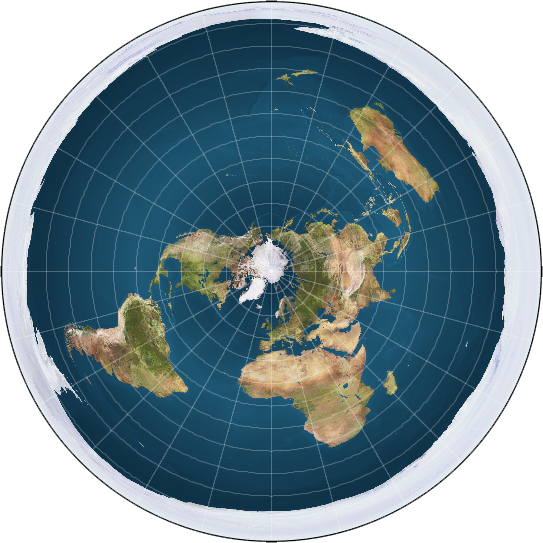
\includegraphics[width=0.9\textwidth]{map.png}\\
			\scriptsize \it PeteSvarrior, for the Flat Earth Wiki; cc-by-sa.
		\end{center}
		\column{0.5\textwidth}
		\large
		Here's a map of a flat earth from the Flat Earth Wiki (ugh).
		
		\BS
		
		The distances are more or less right for the Northern Hemisphere...
		
		\pause
		
		\BS
		\bf They're completely absurd for the Southern Hemisphere!
		
		\BS
		\rm Clearly no Flat Earthers asked any Argentinians how far it was to New Zealand...
	\end{columns}
}

\frame{\frametitle{\textbf{Cherry-picking, examples: reporting bias}}
	\begin{center}
		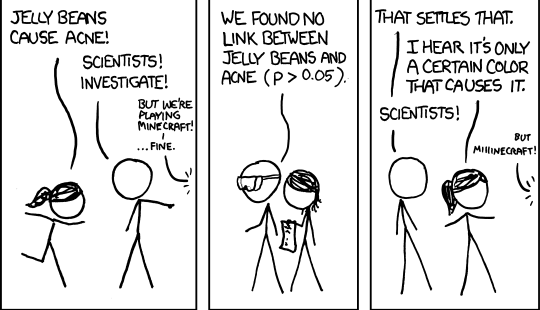
\includegraphics[width=0.8\textwidth]{significant1.png}\\
		$p > 0.05$: ``whatever we found, there's more than a 5\% chance that it is just a coincidence''
	\end{center}
}
\frame{\frametitle{\textbf{Cherry-picking, examples: reporting bias}}
	\begin{center}
		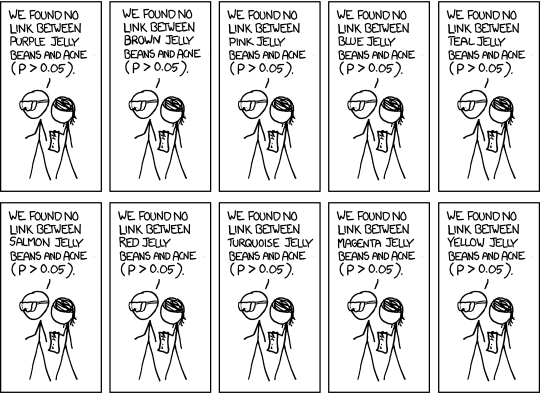
\includegraphics[width=0.8\textwidth]{significant2.png}
	\end{center}
}
\frame{\frametitle{\textbf{Cherry-picking, examples: reporting bias}}
	\begin{center}
		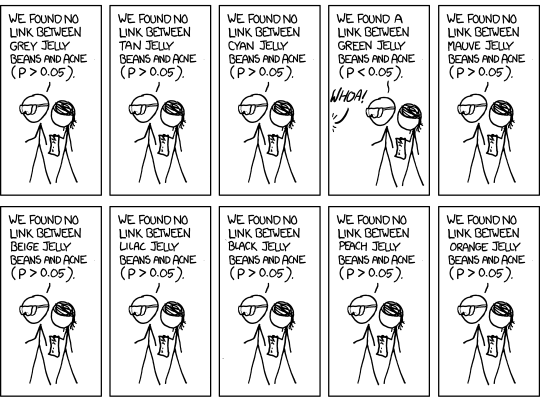
\includegraphics[width=0.8\textwidth]{significant3.png}
	\end{center}
}
\frame{\frametitle{\textbf{Cherry-picking, examples: reporting bias}}
	\begin{columns}
		\column{0.5\textwidth}
		\begin{center}
			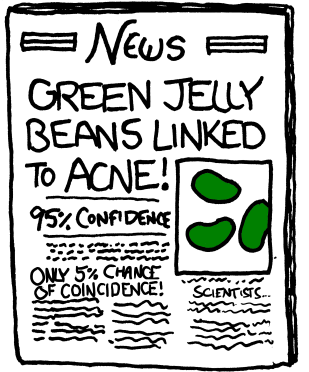
\includegraphics[width=0.8\textwidth]{significant4.png}\\
			\scriptsize \it xkcd \#882, by Randall Munroe: cc-by-nc.
		\end{center}
		\column{0.5\textwidth}
		Laundering data through statistics: dangerous!
		
		\BS
		
		Reporting only an interesting/profitable/exciting piece of data, and ignoring the rest,
		leads to flawed conclusions!
		
		\BS\BS
		
		This is particularly worrying in medical research.
		
	\end{columns}
}


\frame{
	
	\BC
	
	\huge Do you have any favorite examples of biased data causing flawed conclusions? Post to Slack or raise your
	hand and tell me!

\EC

}


\frame{\frametitle{\textbf{Common fallacies: ad hominem arguments}}
	\Large
	
	{\color{Red}{\bf An ad hominem argument} is one that condemns someone else's argument because of {\it who} they are, not 
		the content of their logic.}
	\normalsize
	\BS
	
	\large A few types (paraphrased):
	
	\BS
	\BS
	
	
	Conspiracy-type reasoning (false allegations of ulterior motives):
	\BI
	\normalsize
	\item ``NASA faked the moon landings because they wanted to cover up the fact that their rockets didn't work''
	\item ``The anti-smoking campaign is there to make money, and also something something Nazis'' (\url{http://www.smokingaloud.com})
	\item ``They just {\it say} that fluoride helps dental health but it's really a Communist plot''
	\EI
	
	
	\BS
	\BS
	
	Arguments based on status or identity:
	
	\BI
	\normalsize
	\item ``That person is an esteemed expert; we must trust them without question!''
	\BI
	\item Four out of five dentists recommend such-and-such brand of toothpaste...
	\EI
	\item ``That person is a nobody; how could they have any good ideas?''
	\item ``That person is a member of race/religion/gender/political party XYZ, how could they have anything right to say?''
	\EI
	
}


\frame{\frametitle{\textbf{Ad hominem arguments}}
	\BCC
	\HC
	\BC
	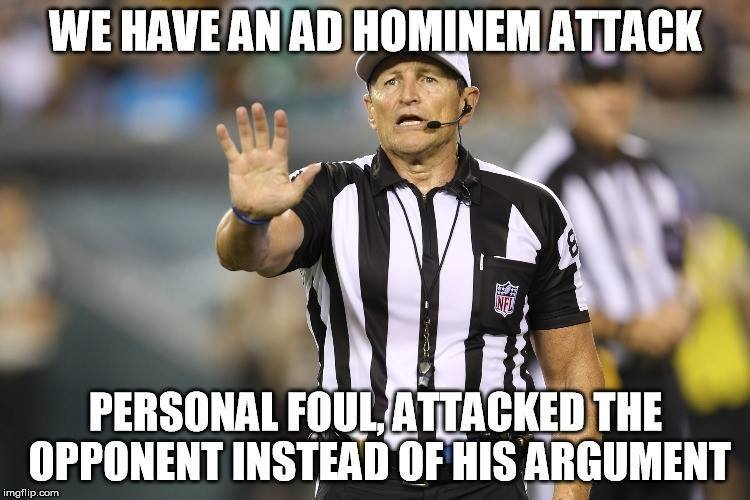
\includegraphics[width=0.8\textwidth]{ad-hom.jpg}
	\EC
	\HC
	{\it Ad hominem} (Latin: ``against the person'') arguments fail the scientific standard of {\it objectivity}:
	claims should be evaluated based on data and logic, not on who is making them.
	
	\BS
	
	False claims of ulterior motives are a common sort of {\it ad hominem} attack.
	
	\ECC
	\BCC
	\HC
	
	\BS\pause
	
	... and using ``argument from authority'' is the reverse: well, if these doctors say that they smoke Camels, they must 
	be safe... right?
	
	\BS
	
	Sometimes deliberately deceptive people really {\it do} have ulterior motives. This can be a warning sign
	that someone is being deceptive...
	\HC
	\BC
	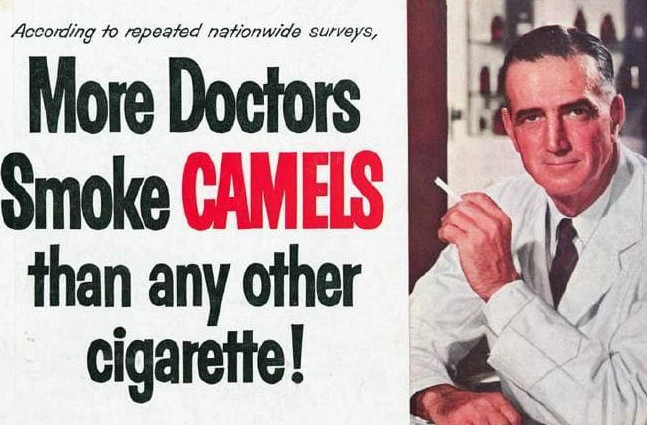
\includegraphics[width=0.8\textwidth]{tobacco-ad.jpg}
	\EC
	\ECC
}


\frame{

\BC

\huge Do you have any favorite examples of arguments from authority or arguments {\it ad hominem}? Post to Slack or raise your
hand and tell me!

\EC
}

\frame{\frametitle{\textbf{Ignoring refuting evidence}}
	
	\BS
	

		{\color{Green} Self-skepticism} is a hallmark of sound science. Good scientists report:
		
		\BI
		\item Any experimental evidence that might conflict with their proposal
		\item All of the possible flaws that {\it they} thought of in their claim
		\BI
		\item ... and how they considered them
		\EI
		\item Any tests that anyone {\it else} could do to try to disprove them
		\item All the things that make them {\color{Red} uncertain} about their result
		\item The limits of their conclusions
		\EI
		

		\BS\BS
		
		Most good scientific writing spends much of its time doing the above. You should only try to convince
		other people you are right once you have 
		tried very hard, yet failed, to prove yourself wrong.
		
		\BS
		
		Any claimant that spends most of their time talking {\it up} their conclusions is likely suspect.
		
	}

\frame{\frametitle{\textbf{Ignoring potentially refuting evidence}}
	\large
	
	{\color{Red}Ignoring or failing to search for refuting evidence} is a common trait of faulty scientific process. 
	This can either be:
	
	\BS
	\BI
	\item Ignoring refuting evidence altogether, even if it's widely known
	\item Dismissing refuting evidence out of hand, without considering it in any real way 
	\item Failing to think of potentially refuting evidence and search for it
	\EI
	\Large
	\BC
	Do you have any favorite examples of flawed scientific claims that fail to address potentially refuting evidence?
	
	\BS
	
	\large
	\EC
	
	\large
	
	\BS
	\BS
	\BC
	\url{https://wiki.tfes.org/Flat_Earth_-_Frequently_Asked_Questions}
	\EC
	
}

\frame{\frametitle{\textbf{Manufacturing a controversy}}
	\large
	We've discussed some of the common features of people {\it advancing scientific claims}
	incorrectly, negligently, or dishonestly.
	
	\BS
	\BS
	
	Sometimes dishonest people aren't trying to {\it advance} something they know to be false, though.
	
	\BS
	
	They're more interested in convincing people to {\it reject} something that is true.
	
	\BS
	
	To do that, they only need to create doubt. This is commonly done by {\it manufacturing a controversy}.
	
	\BS\pause
	
	\BS\BS
	\normalsize
	
	(This is a common tactic to erode trust in {\it anything}, not just science -- common in politics and negative advertising)
}

\frame{\frametitle{\textbf{Manufacturing a controversy}}
	
	\Large
	\BC
	Do you have any favorite examples of manufactured controversies?
	\EC
	
	\pause
	
	Consider again the tobacco industry:
	
	\BI
	\item ``Secondhand smoke doesn't cause health problems; those studies are wrong''
	\item ``Are you really sure that secondhand smoke causes health problems? Maybe it was building ventilation!''
	\EI
	
	One of these is a far easier sell than the other!
	
	\BS
	\BS
	\normalsize
	{\it The industry's strategy does not require winning the debates it manufactures. It is enough to foster and perpetuate the illusion of controversy in order to muddy the waters around scientific findings that threaten the industry. Thus it offers reassurance to smokers, helping them to rationalize and repress their health concerns. Furthermore, claims of ``not proven'' resonate with friendly or naive journalists and governments, and provide an excuse for not taking strong governmental or societal action against tobacco.}
	
	\scriptsize
	\BS
	\begin{flushright}--Yussuf Saloojee and Elif Dagli,  "Tobacco industry tactics for resisting public policy on health" Bull. World Health Organ. 78(7): Genebra, July 2000.\end{flushright}
}



\frame{\frametitle{\textbf{Sensationalism}}
	\Large
	Two things are both true:
	
	\BI
	\item Some scientific findings can dramatically change our lives and our perspective on the world, and are compelling and exciting
	\item Whether a scientific claim is true or not doesn't depend on whether it's exciting or not (objectivity)
	\EI
	
	\BS\BS
	
	Scientists thus have twin duties:
	
	\BI
	\item They should engage with society in sharing the excitement and interest of their findings. Science communication is vital (and many of us are bad at it; the astronomers do better than the physicists!)
	\item They should {\color{Red} separate this excitement} from the task of {\color{Green} evaluating the validity of claims}
	\EI
}

\frame{\frametitle{\textbf{Sensationalism}}
	\large
	Beware of any sort of scientific claim that conflates {\color{Red}the evidence that it is true} with {\color{Green}why you should be excited by it}, or that seems to be {\color{D}hyped by its claimant}.
	
	\BS
	\BS
	
	Good scientists do hold press conferences, because many discoveries are exciting!
	
	\BS
	
	But these happen only in the context of:
	
	\BI
	\item a vast amount of self-skepticism applied to their results first
	\item objective, sober presentation of the {\it evidence} for their conclusions
	\EI
	

}

\frame{\frametitle{\textbf{Science vs. pseudoscience}}
\BC\Large
Often people adopt the trappings of science to give nonscientific ideas a veneer of validity.
This is called ``pseudoscience'' -- fake science.
\EC

\begin{columns}

\column{0.5\textwidth}
\color{Green}
\Large \BC Science \EC
\large
\BI
\item Universal models
\item Natural principles
\item Testable predictions
\item Not anthropocentric
\item Replicable results
\item Self-skepticism
\EI

\column{0.5\textwidth}
\color{Red}
\Large \BC Pseudoscience\EC
\large
\BI
\item Singular events
\item Supernatural explanations
\item Untestable predictions
\item Different rules for people
\item Results defy replication
\item Self-promotion
\EI
\end{columns}
}

%
%\frame{
%\BC
%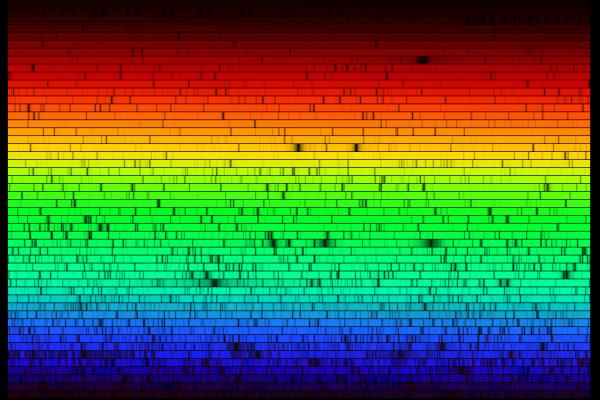
\includegraphics[width=0.9\textwidth]{solarspectrum.jpg}
%\large
%
%This is a ``picture'' of the Sun. What can we learn from it?
%\EC
%}

%\frame{
%
%\large
%\BC
%How much of the light in this room can you see?\EC
%
%\BS\BS
%\Large
%\color{A}A: All of it\\
%\color{B}B: Most of it \\
%\color{C}C: Around a quarter of it\\
%\color{D}D: Not much of it at all\\
%}
%
%\frame{
%\large
%\BC
%\large
%How much of the sound in this room can you hear?\EC
%\Large
%\BS\BS
%
%\color{A}A: All of it\\
%\color{B}B: Most of it \\
%\color{C}C: Around a quarter of it\\
%\color{D}D: Not much of it at all\\
%}
%
%\frame{
%\large
%\BC
%Sounds can have a spectrum of frequencies and wavelengths, 
%and we can only perceive a piece of that spectrum.
%
%\BS\BS\pause
%
%\BS
%
%In the same way {\it light} has a spectrum of frequencies/wavelengths, 
%and our eyes only perceive a tiny fraction of that spectrum.
%
%\color{Red}
%When we say ``light'', we mean {\it all} wavelengths, not just the 
%ones we can see!
%\EC
%}
%
%\frame{\frametitle{\bf The electromagnetic spectrum}
%
%\BC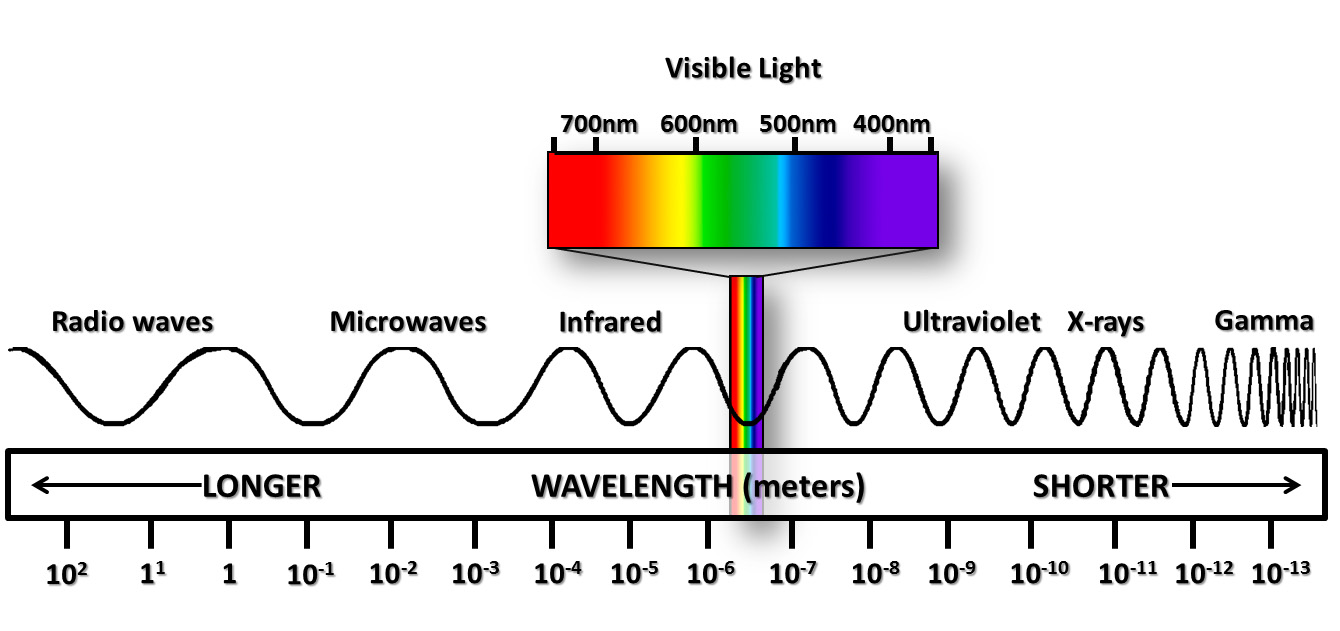
\includegraphics[width=0.8\textwidth]{linear-spectrum.jpg}
%
%\BS
%
%There is an enormous range of ``colors'' of light out there!\EC
%
%\BS\BS
%
%What's this ``sound'' like?
%
%\pause
%\BS
%{Music: ``The Blood of Cu Chulainn'', from the soundtrack to {\it Boondock Saints} (Jeff Danna, 1999)}
%
%\BS\pause
%
%We can learn far more about what's going on in the orchestra if we 
%have the whole spectrum, rather than just a piece!
%}
%
%\frame{
%\BC
%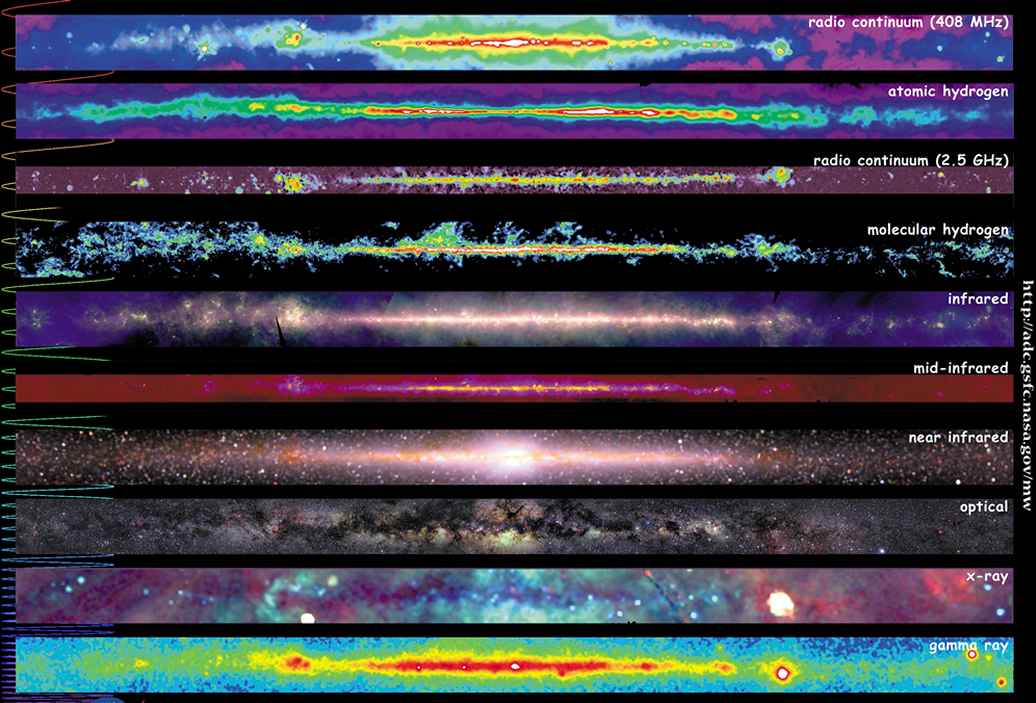
\includegraphics[height=0.9\textheight]{mwmw.jpg}
%\EC
%}
%
%
%
%\frame{\frametitle{\bf{An illuminating story}}
%
%In the late 19th century, the laws of electromagnetism looked like this:
%
%\BI
%\item Electric fields exert a force on electric charges
%\item Magnetic fields exert a force on {\it moving} electric charges
%\EI
%
%\bigskip
%
%We know this thanks in large part to the work of Michael Faraday, who
%famously wasn't good at algebra and drew pictures of fields.
%
%\bigskip
%
%Where do these fields come from?
%
%\BI
%\item Electric charges make electric fields
%\item Moving electric charges make magnetic fields
%\item Changing magnetic fields make electric fields
%\pause
%\item {\color{Red} Changing electric fields make magnetic fields}
%\EI
%}
%
%\frame{\frametitle{\bf{An illuminating story}}
%
%\BI
%\item Electric charges make electric fields
%\item Moving electric charges make magnetic fields
%\item Changing magnetic fields make electric fields
%\item {\color{Red} Changing electric fields make magnetic fields}
%\EI
%
%\BS
%
%Last law added by James Clerk Maxwell in the 1860's, and it has
%a surprising consequence:
%
%\BS
%\BI
%\item{Changing electric field makes a magnetic field}
%\pause \item ... which makes a magnetic field ...
%\pause \item ... which makes an electric field further away ...
%\pause \item This leads to a traveling electromagnetic disturbance: an {\it electromagnetic wave}.
%\EI
%}
%
%\frame{\frametitle{\bf{An illuminating story}}
%
%Maxwell calculated that these electromagnetic waves traveled at
%around 300 million meters per second.
%
%\BS
%
%Independently, light had been measured to travel at 300 million
%meters per second some years prior.
%
%\BS \pause
%
%So ... if this electromagnetic wave travels at the speed of
%light, perhaps it {\it is} light?
%
%\BS
%
%In the history of science, sometimes theory gets ahead of experiment -- like in the discovery of the nature of light.
%}
%


\end{document}
